\usetikzlibrary{arrows.meta}
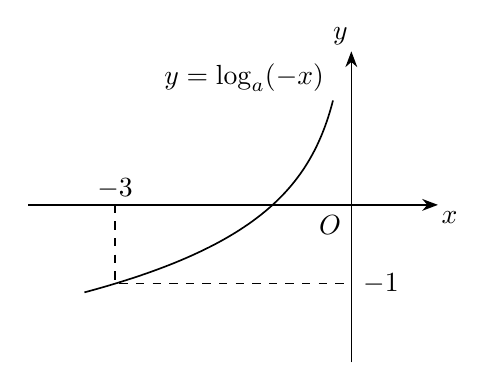
\begin{tikzpicture}[x=1cm,y=1cm,line width=.6pt,>=Stealth,font=\normalsize]
\draw[->] (-4.10,0) -- (1.10,0) node[below right,inner sep=0pt,xshift=1pt,yshift=-2pt] {$x$};
\draw[->] (0,-2.00) -- (0,1.95) node[above left,inner sep=0pt,xshift=-1pt,yshift=2pt] {$y$};
\draw[dashed] (-3,0) -- (-3,-1) -- (0,-1);
\draw[domain=0.233:3.39,samples=160] plot ({-\x},{-ln(\x)/ln(3)});
\node[anchor=north east,inner sep=0pt] at (-0.12,-0.12) {$O$};
\node[anchor=south,inner sep=0pt,yshift=2pt] at (-3,0) {$-3$};
\node[anchor=west,inner sep=0pt,xshift=4pt] at (0,-1) {$-1$};
\node[anchor=south east,inner sep=0pt,xshift=-3pt,yshift=3pt] at (-0.233,1.325674) {$y=\log_a(-x)$};
\end{tikzpicture}
